%%%%%%%%%%%%%%%%%%%%%%%%%%%%%%%%%%%%%%%%%%%%%%%%%%%%%%%%%%%%%%%%%%%%%%%%
\chapter{Robust networks}
\label{ch:robust-networks}
%%%%%%%%%%%%%%%%%%%%%%%%%%%%%%%%%%%%%%%%%%%%%%%%%%%%%%%%%%%%%%%%%%%%%%%%

In this chapter we describe the experiments that I did during my thesis
work. See Chapter \ref{ch:background} for a rationale of what we're
going to. Section \ref{sec:number-of-epochs}
is dedicated to how the models have been trained and how the number of
epochs of training has been chosen, Section
\ref{sec:deploying-a-filtering-technique} talks about how I
\emph{deployed} a filtering technique over an existing model and how I
made that choice, and finally Section \ref{sec:better-than-pca} is
dedicated to a comparison of the different filtering techniques and
which is the one that ended up to perform better as a defense against
adversarial examples.

\section{Number of epochs}
\label{sec:number-of-epochs}

As we started to test the performance of various setups we were
basically generating a lot of different models that had to be trained
first, before running experiments on them. Each one had different
characteristics and different rates of learning so fixing a pre-defined
number of epochs to train every model for might have been resulted in
comparing models with very different accuracies: as explained in
Chapter \ref{ch:background} the accuracy has a direct impact on the
resiliency of the model against adversarial examples --- that would
have been make a filter technique win even if the real reason for that
result was a low accuracy. One choice would have been to choose a
predefined accuracy for all the models to reach but choosing a too low
value would have been resulted in unrealistic measurements (no one
wants to use models with accuracy lower than 40\% for example) while
choosing a high value for the accuracy had the risk of potentially
being unreachable for some models.

The approach that we decided to use to somewhat solve this problem was
to come up with \emph{heuristics} to decide whether a model has
stopped learning or not. It's not perfect: models will still reach
different accuracies. But hopefully they will be all closer. The number
of epochs is then defined dynamically as the model trains.

As we wanted to test models with the highest possible accuracy that we
can make them reach we made the model reduce the learning rate
(see Chapter \ref{ch:background}) when the accuracy of the model didn't
seem to improve anymore. In fact, ``models often benefit from reducing
the learning rate by a factor of [2 up to 10 times] once learning
stagnates''\footnote{https://github.com/keras-team/keras/blob/2ad932b/keras/callbacks.py\#L991-L992}.

Now, the heuristics we chose were:
\begin{enumerate}
  \item stop learning after the accuracy does no longer improve over a
    specified number of epochs
  \item stop learning after the model's weights are pretty stable over a
    specified number of epochs
\end{enumerate}

Note that both the heuristics wait after a ``specified number of
epochs" to make their decision. We're calling this value the
\emph{patience}, as that's the amount of \emph{time} the heuristic take
before making its final decision.

To prove that both the heuristics work and to choose the one that
worked better I decided to stick with a single model of which we assume
to more or less know the number of epochs needed to reach an accuracy
of 97\% and see if we can reach that same accuracy even without
specifying the number of epochs but relying only on the heuristics to
stop training. Throughout the codebase we called this setting training
the model for a number of epochs equals to -1.

The model used is a feedforward network of two layers of 100 hidden
neurons each and ten output neurons. I'm going to call it
\texttt{fc-100-100-10} for obvious reason throughout the rest of the
document. In \cite{bhagoji2018enhancing}, Princeton researchers trained
that model for 500 epochs achieving an accuracy of circa 97.5\%. That's our
baseline.

\subsection{Early stopping heuristic}
This heuristic is already implemented by Keras as a callback to the
learning phase\footnote{https://keras.io/callbacks/\#earlystopping}. It
checks if over the patience a chosen metrics has stopped improving. If
that happens we deduce the model stopped training. We set a patience of
60 epochs as on our Google Cloud Platform machine 60 epochs corresponds
to a whole minute.

\subsection{Stop on stable weights heuristic}
We implemented this heuristic from scratch. Data on model weights are
collected. Taking the weight that has the largest standard deviation
over the patience, if that standard deviation is below a certain
threshold, according to the heuristic, the model has stopping learning
and getting stable. Again, we set a patience of 60 epochs.

\subsection{Data obtained}

\begin{figure}
  \centering
  \begin{tabular}{|c|c|c|}
    \hline
    & fixed lr & reduce lr \\
    \hline
    early stopping & 97.44\% & 97.18\% \\
    \hline
    stable weights & 97.66\% & 97.6\% \\
    \hline
  \end{tabular}
  \caption{Accuracies when training with different techniques}
  \label{fig:accuracy-heuristics}
\end{figure}

Our baseline was that of \texttt{fc-100-100} trained for 500 epochs
reaching an accuracy of 97.55\%. To check how stable was that accuracy
we trained the same network for another 500 epochs reaching an accuracy
that was only slightly higher --- 97.71\%. Reducing the learning rate
on plateau instead decreased the accuracy to 97.47\%, both for 500
epochs and 1000 epochs. That said, as we planned to let our models
train until an heuristics decides to stop it we thought longer training
sessions would not be our main problem for our future
experiments\footnote{Actually there's another problem: that the model
  escapes the plateau but the accuracy of the model grows so slowly
  that an heuristic will block its training as it thinks it's
  \emph{converging}. Using the heuristic of stopping training when
  model's weights are stable should keep away this situation}.

You can see results in Figure \ref{fig:accuracy-heuristics}. The
combination that seemed to work better was to stop training on model's
stable weights, keeping the learning rate fixed, getting a final
accuracy of 97.66\%. That said, as the difference between using a fixed
value for the learning rate or reducing that on plateau was not that
distinct and given that the reducing the learning rate intuitevely felt
useful in the general
case\footnote{https://datascience.stackexchange.com/questions/37163/is-it-a-good-practice-to-always-apply-reducelronplateau-given-that-models-b/37190}
we chose to reduce the learning on plateau. We understand the decision
is rather arbitrary but we chose that. As for the heuristics we chose
to stop training on stable weights.

In the following sections all the models considered have been trained
using this setup then. That is, training for an undefined number of
epochs, stopping when the model's weights become stable --- i.e. the
related standard deviation reach a value under a threshold of 0.5 over
60 epochs --- reducing the learning rate after a plateau of 30 epochs.

\section{Deploying filters}
\label{sec:deploying-filters}

When testing different filter tecniques just \emph{finding the right
  one} is not enough. In fact how do you \emph{deploy} that filter
technique in your model is something you have to choose. For example
you can add your filtering technique to the data pipeline \emph{before}
training and let the model train on filtered input.

We had a couple of alternatives here and we had to measure their
different performance in order to choose which one was the better fit
for our work.

We identified at least two different fashions to integrate a filter
technique in our models. We can either add a filter layer to a model
already trained on unfiltered input, or we can add a layer to an
already trained model and retrain the network for some epochs after
this layer has been added. Basically the difference is that in the latter case, the model has
been trained only on filtered input.
Inspired by lexicon used in \cite{bhagoji2018enhancing}, we named the
first technique as \emph{reconstruction} and the second one
\emph{retraining}.\footnote{There's another alternative which is to
  initialize the model, add the filter layer then train the network
  while it's still \emph{untouched}. It basically consists in making
  the network never to see unfiltered input. This seemed to make things
  so much better for the attacker than both reconstruction and
  retraining that we just avoided to compare it with the other
  approaches.}

We did some measurements to better understand which technique was
better was not that clear.

We took the same model --- \texttt{fc-100-100-10} --- and deployed the
PCA\footnote{https://en.wikipedia.org/wiki/Principal\_component\_analysis}
filter technique using both reconstruction and retraining. Changing
the number of components retained (see Chapter \ref{ch:background}) we
obtained dozens of models and trained all them leveraging the
heuristics described in Section
\ref{sec:dynamically-choosing-the-number-of-epochs}.

We attacked each model using the fast gradient sign technique (see
Chapter \ref{ch:background}) obtaining what was the adversarial success
score given the value of $\eta$\footnote{As explained in Chapter
  \ref{ch:background}, $\eta$ is the the freedom given to the attacker:
  the more the freedom the easier is to forge an input.}.

Then we compared the adversarial success score for each model trained
using reconstruction to the attacker performance on the same model now
built using retraining. By subtracting these two values, making an
average for each models pair and finally making an average for all the
pairs, we got what was the average gain (or loss) in the model's
resiliency for reconstruction over retraining.

We wrote a script \texttt{retraining-versus-reconstruction.py}
implementing the comparison described above and we obtained that
retraining is only 1\% more effective than reconstruction. This is a
rather disappointing result. In fact, as implementing retraining
consistently throughout the codebase was harder than to stick with
reconstruction given the results we decided it was not worth the effort
and we abandoned retraining.

For this reason in the following sections we will talk only about models
with filter techniques deployed using reconstruction.

\section{Filters better than PCA}

In this chapter we'll test a couple of image filters against
adversarial input. The intuition behind the idea of filtering the image
is that to forge an adversarial input the attacker will try to put some
noise distributed in the image. Trying to be stealthy the noise will be
hidden to a human eye. As these filters highlight the \emph{important}
features of an image, that is more or less what an human eye sees, we
hope they cut out the noise introduced by the attacker. Intuitevely,
the more the attacker wants to be stealthy the more these filters are
likely to succeed in deleting the attacker noise.

The idea is taken from \cite{bhagoji2018enhancing} in which a \emph{PCA
  filter} (that is a filter obtained applying a PCA transformation then
its inverse, as explained in Section \ref{sec:sklearn}) is applied to
the input of a feedforward neural network aiming to reduce the
probability of success for an attacker forging adversarial examples
against the model. We'll take this idea further by using a
decomposition technique other than PCA: hopefully other filters will
work better.

\begin{figure}
  \centering
  \begin{subfigure}{0.3\linewidth}
    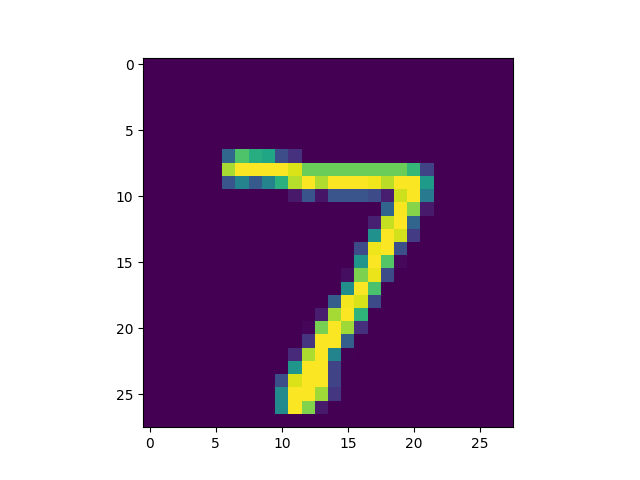
\includegraphics[width=\linewidth]{filtered-input-pca-784-components.png}
    \caption{784 components}
  \end{subfigure}
  \begin{subfigure}{0.3\linewidth}
    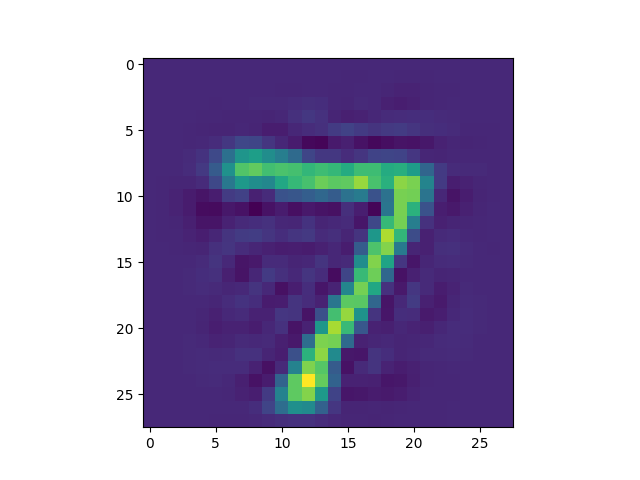
\includegraphics[width=\linewidth]{filtered-input-pca-100-components.png}
    \caption{100 components}
  \end{subfigure}
  \begin{subfigure}{0.3\linewidth}
    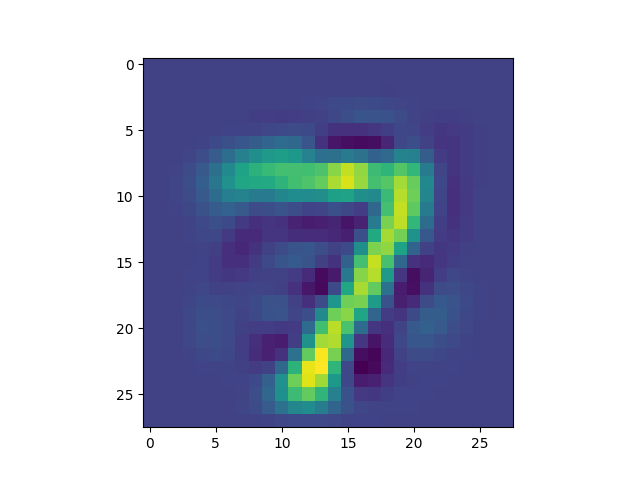
\includegraphics[width=\linewidth]{filtered-input-pca-40-components.png}
    \caption{40 components}
  \end{subfigure}
  \caption{Retaining a different number of components for a PCA filter.}
  \label{fig:various-pca-reductions}
\end{figure}

Just like PCA and as already explained in Chapter \ref{ch:background}
each of these decomposition techniques can be more or less destructive
in regards of the original image. Intuitevely these filters, like PCA,
\emph{decompose} the original image of $n$ pixels into a vector of less
than $n$ components. From this vector it is possible to reverse the
decomposition operation obtaining again an image of $n$ pixels but
starting from a smaller amount of information the portion of
information lost is \emph{interpolated}. For example in Figure
\ref{fig:various-pca-reductions} a decreasing number of components is
retained, that is a decreasing amount of information of the original
image is kept --- the rest is interpolated using an inverse function of
the PCA transformation. Notice how the quality of the image degrates
making the number 7 less and less recognizible but the feature of the
number 7 are the ones that survive the most. That happens both for the
human eye and the model.

The idea is to find a balance between this degradation that will slowly
remove the features that allow to recognize the number 7 and remove the
noise maliciously introduced by the attacker. Intuitively the more
invasive the filter the better will be the defense. Unfortunately the
better the defense the more the lost accuracy too: two different images
can be confused as the same image for the model as the information that
distiguished the two images is now potentially lost. That means that
the \emph{best} filter will be the one that provides the best defense
given the accuracy lost by the model is not \emph{too much}.

\begin{figure}
  \centering
  \begin{subfigure}{0.3\linewidth}
    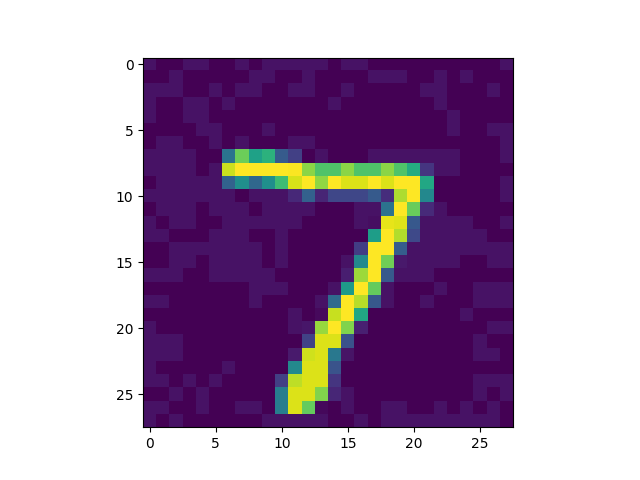
\includegraphics[width=\linewidth]{adversarial-input-fc-100-100-10-005.png}
    \caption{$\eta = 0.05$}
  \end{subfigure}
  \begin{subfigure}{0.3\linewidth}
    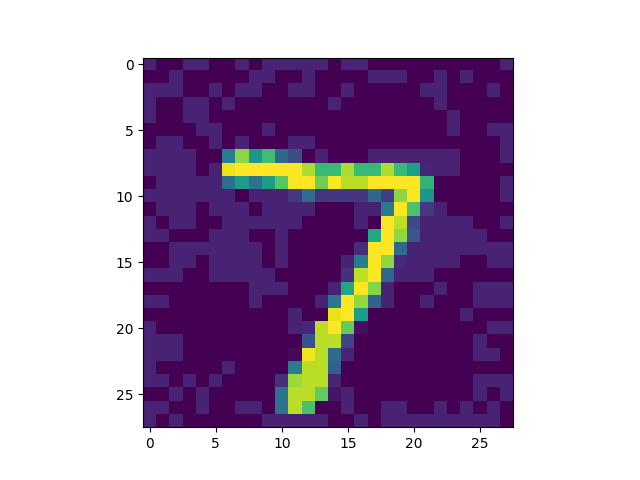
\includegraphics[width=\linewidth]{adversarial-input-fc-100-100-10-01.png}
    \caption{$\eta = 0.1$}
  \end{subfigure}
  \begin{subfigure}{0.3\linewidth}
    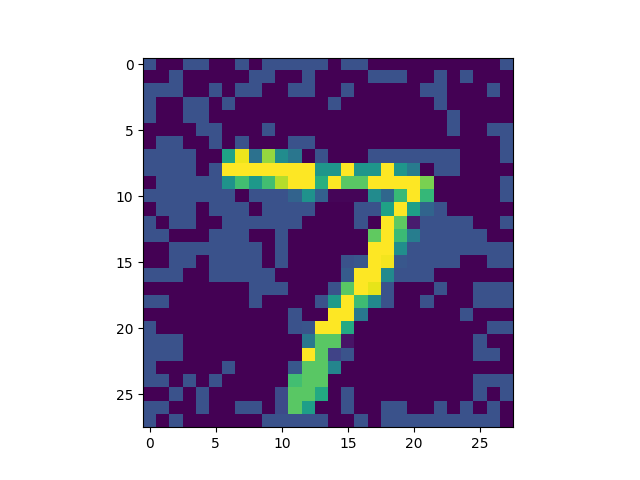
\includegraphics[width=\linewidth]{adversarial-input-fc-100-100-10-025.png}
    \caption{$\eta = 0.25$}
  \end{subfigure}
  \caption{Adversarial examples as $\eta$ increases.}
  \label{fig:fgs-increasing-eta}
\end{figure}

The attack used is called Fast Gradient Sign. As it has been already
described in Chapter \ref{ch:background}, the attacker can be more or
less stealthy by choosing a higher or lower value for $\eta$
respectively --- see Figure \ref{fig:fgs-increasing-eta}. This makes
Fast Gradient Sign a parameterized attack, meaning that studying which
filter is more resilient to attacks would require us to use different
values of $\eta$.

As that would make the number of cases to study
combinatorically explode we decided to fix a value of $\eta$ to 0.1 and
consider fast gradient sign as a single type of attack with no
parameters. 0.1 has been chosen as it's a median value
between a completely ineffective attack of $\eta$ equals to 0 and an
attack that's detectable by a human eye --- that is, $\eta$ equals
to 0.25.

In our gray-box setting (see Chapter \ref{ch:background}) we measured
an accuracy on the MNIST test set of 97.39\% and an adversarial success
score --- that is, the probability of success for the attacker --- of
81\%. We expect the latter to go down as we increase the degree
to which the filter technique is destructive. Yet as we try to stop the
attacker we have to reduce the accuracy of the model as well.

\section{Decompositions}

When it comes to testing various filtering techniques we had two
choices: implementing them from scratch using TensorFlow --- as we did
at first with PCA --- or we could leverage the \texttt{decomposition}
module of
sklearn\footnote{http://scikit-learn.org/0.20/modules/classes.html\#module-sklearn.decomposition}.
As explained in Chapter \ref{ch:tools-and-libraries} to derive a filter
from a decomposition technique we need to have both the transformation
function --- that performs the dimensionality reduction that names the
class --- and its inverse function. \texttt{sklearn.decomposition}
implements the former for all of its classes but the related inverse
function is not always available.

\begin{figure}
  \centering
  \begin{tabular}{|c|c|}
    \hline
    Decomposition technique & Inverse function\\
    \hline
    \texttt{DictionaryLearning} & no \\
    \hline
    \texttt{FactorAnalysis} & no \\
    \hline
    \texttt{MiniBatchDictionaryLearning} & no \\
    \hline
    \texttt{MiniBatchSparsePCA} & no \\
    \hline
    \texttt{SparsePCA} & no \\
    \hline
    \texttt{SparseCoder} & no \\
    \hline
    \texttt{FastICA} & yes \\
    \hline
    \texttt{IncrementalPCA} & yes \\
    \hline
    \texttt{KernelPCA} & yes \\
    \hline
    \texttt{NMF} & yes \\
    \hline
    \texttt{PCA} & yes \\
    \hline
    \texttt{TruncatedSVD} & yes \\
    \hline
  \end{tabular}
  \caption{Decomposition techniques implemented by sklearn 0.20}
  \label{fig:decomposition-techniques}
\end{figure}

As shown in Figure \ref{fig:decomposition-techniques} of 16
decomposition techniques implemented in \texttt{sklearn.decomposition}
only half of them have the inverse function implemented, or defined
--- I guess that for some of them the inverse function does not even
exist, but didn't make any research on that.

Of course each of these transformers had been \emph{fitted}, as the
function they compute is dependent on the dataset you're going to use.
For example, to do PCA filtering on the MNIST dataset you need to fit
the transformer on the MNIST dataset. This required time and some
transformers --- namely the KernelPCA --- didn't succeeed in fitting,
failing to \emph{converge} : I had to discard them even if they had an
inverse function.

Once transformers has been fitted we can add them as a preprocessing
layer in the models in a \emph{reconstruction} fashion --- as explained
in Section \ref{sec:deploying-a-filtering-technique}.

\section{Better than PCA}

Now we're ready to answer the question that motivated the thesis ---
see Chapter \ref{ch:background}. That is, we started from the work in
\cite{bhagoji2018enhancing} where a PCA filtering technique has been
proposed as a defense against adversarial examples. We want to find out
if we can find some filter technique that works better than PCA.

Answering this question required a bit of reasoning. In fact, defining
what's \emph{better} than PCA wasn't straightforward, especially since
models using with different filter technique had different
accuracy and comparing all the models together would result in
priviledging the models with a low accuracy --- as the lower the
accuracy the harder is for the attacker to forge adversarial examples.

So instead of defining an index that would compute a score of the
defense provided by the filter somehow weightening the accuracy of the
model --- which we did at first ---, we decided to partition the models
in intervals of accuracy and tried to find the best filter restricted
to that interval.

\begin{figure}
  \centering
  \begin{tabular}{|c|c|c|c|c|}
    \hline
    $\approx$accuracy & filter & accuracy & adversarial score\\
    \hline
    \hline
    97.39\% & TruncatedSVD & +0.02\% & -11\% \\
    \hline
    97.36\% & PCA & N/A & N/A \\
    \hline
    97.32\% & IncrementalPCA & +0.02\% & -0.05\% \\
    \hline
    97.17\% & NMF & -0.17\% & -1.6\% \\
    \hline
    93.8\% & PCA & N/A & N/A \\
    \hline
  \end{tabular}
  \caption{Comparing filter performances in respect to PCA.}
  \label{fig:filters-comparison}
\end{figure}

What we did find is that it's hard to improve over PCA. The performance
of the other filters is very similar to the performance of PCA, as
shown in Figure \ref{fig:filters-comparison}. The only interesting
improvement is for using TruncatedSVD on a model whose accuracy is of
circa 97.39\%; in fact, we registered an improvement of 11\% over the
adversarial score for the same model defended by a PCA filter.
